% !TEX root = main.tex
% !TEX root = main.tex
\documentclass[10pt]{beamer}
\usetheme{Boadilla}
\usefonttheme{default}
\usecolortheme{beaver}


% Mathematical symbols
\usepackage{amsmath,amsfonts,amssymb,amsthm,mathtools} % for formatting and enhancing mathematical notation and equations


% Images
\usepackage{graphicx} % for working with images
\graphicspath{{image/}}
\usepackage{tikz} % for creating graphics and diagrams directly 
\usetikzlibrary{calc}
\usepackage{floatrow} % provides additional control over figure and table placement, 
                      % including the [H] option for precise figure placement
\usepackage[margin=10pt,font=small,labelfont=bf,labelsep=period]{caption} % to configure 
                                    % the appearance of captions for figures and tables
%\usepackage{lipsum} % for generating placeholder text


% Tables
\usepackage{array} % for creating arrays and matrices within mathematical environments
\usepackage{tabularx} %  provides an environment for creating tables with columns of 
                      %  varying widths that automatically adjust to fit the content
\usepackage{tabulary} %  similar to the previous one
\usepackage{booktabs} %  enhancing readability and aesthetics
\usepackage{longtable} %  for creating tables that can span multiple page


\usepackage{hyperref} % for adding links and customizing them
\hypersetup{
	colorlinks=true,        % false: boxed links; true: colored links
	linkcolor=black,        % Color of internal links (e.g., table of contents)
	citecolor=refcolor,     % Color of citation links
	urlcolor=refcolor       % color of external links
}

\usepackage{biblatex} % bibliography-management package


%Custom colors
\definecolor{titlecolor}{RGB}{208,0,5}
\definecolor{refcolor}{RGB}{164,16,26} 
\definecolor{itemcolor}{RGB}{164,16,26}

\definecolor{foot1}{RGB}{240,166,166}
\setbeamercolor{color1}{fg=black,bg=foot1}

\definecolor{foot2}{RGB}{246,211,211}
\setbeamercolor{color2}{fg=black,bg=foot2}

\definecolor{foot3}{RGB}{240,223,223}
\setbeamercolor{color3}{fg=black,bg=foot3}

\definecolor{foot4}{RGB}{230,230,230}
\setbeamercolor{color4}{fg=black,bg=foot4}

%\definecolor{alertcolor}{RGB}{255,0,0} % Red for alerts
%\definecolor{boxcolor}{RGB}{0,128,0}  % Green for boxes
%\definecolor{examplecolor}{RGB}{0,0,255}  % Blue for example boxes


%Change colors
\setbeamercolor{titlelike}{parent=palette primary,fg=titlecolor}
\setbeamercolor{item}{fg=itemcolor}

%\setbeamercolor{alerted text}{fg=alertcolor}

%\setbeamercolor{block title}{bg=boxcolor, fg=white}
%\setbeamercolor{block body}{bg=white, fg=black}

%\setbeamercolor{block title example}{bg=examplecolor, fg=white}
%\setbeamercolor{block body example}{bg=white, fg=black}

%\setbeamercolor{block title alerted}{bg=alertcolor, fg=white} %
%\setbeamercolor{block body alerted}{bg=white, fg=black} 


%Footline
\setbeamertemplate{footline}{
\begin{beamercolorbox}[wd=\paperwidth,ht=2.25ex,dp=1ex,left]{color1}%
	\begin{beamercolorbox}[wd=0.3\paperwidth,ht=2.25ex,dp=1ex,center]{color1}%
		\insertshorttitle
	\end{beamercolorbox}%
	\begin{beamercolorbox}[wd=0.3\paperwidth,ht=2.25ex,dp=1ex,center]{color2}%
		\hspace*{5ex} \insertshortauthor
	\end{beamercolorbox}%
	\begin{beamercolorbox}[wd=0.3\paperwidth,ht=2.25ex,dp=1ex,center]{color3}%
		\hspace*{5ex} \insertshortdate
	\end{beamercolorbox}%
	\begin{beamercolorbox}[wd=0.1\paperwidth,ht=2.25ex,dp=1ex,center]{color4}%
		\hspace*{1ex} \insertframenumber{} / \inserttotalframenumber
	\end{beamercolorbox}%
\end{beamercolorbox}%
} 


% Define the \box and \myboxmath commands with the custom color
\usepackage{tcolorbox} 
\newtcbox{\mybox}{on line,colback=white,colframe=refcolor,size=fbox,arc=3pt,boxrule=0.8pt}
\newcommand{\myboxmath}[1]{\mybox{$#1$}}


%The next block of commands puts the table of contents at the 
%beginning of each section and highlights the current section:
%\AtBeginSection[]
%{
%  \begin{frame}
%    \frametitle{Table of Contents}
%    \tableofcontents[currentsection]
%  \end{frame}
%}

% Remove the navigation bar from slides
\beamertemplatenavigationsymbolsempty 

% Enable numbering of figures and tables in captions
\setbeamertemplate{caption}[numbered]

% Adjust captions
\usepackage{caption}
\captionsetup[figure]{font=small,skip=0pt}
 
\addbibresource{include/references.bib} % Import the bibliography file
% !TEX root = main.tex

\title[ FH-PS-AoP Challenge]{Pubic Symphysis-Fetal Head Segmentation \\
and Angle of Progression}
\subtitle{Grand Challenge Review}
\author[Anna Putina]{Anna Putina}

\institute[FIB UPC]
{
  Facultat d’Informàtica de Barcelona,\\
 
Universtat Politècnica de  Catalunya

}

\date[November 28th, 2023] 
{November 28th, 2023}

%\logo{\includegraphics[height=1cm]{image/logo}}





\begin{document}

%The next statement creates the title page
\frame{\titlepage}

%---------------------------------------------------------
%This block of code is for the table of contents after
%the title page
\begin{frame}
    \frametitle{Table of Contents}
    \tableofcontents
    \end{frame}
%---------------------------------------------------------

\section{Clinical Background and Data}

\begin{frame}
    \frametitle{Clinical Background and Data}
\begin{columns}
    \column{0.5\textwidth}
    \vspace{-4mm}
    \begin{figure}[H]
        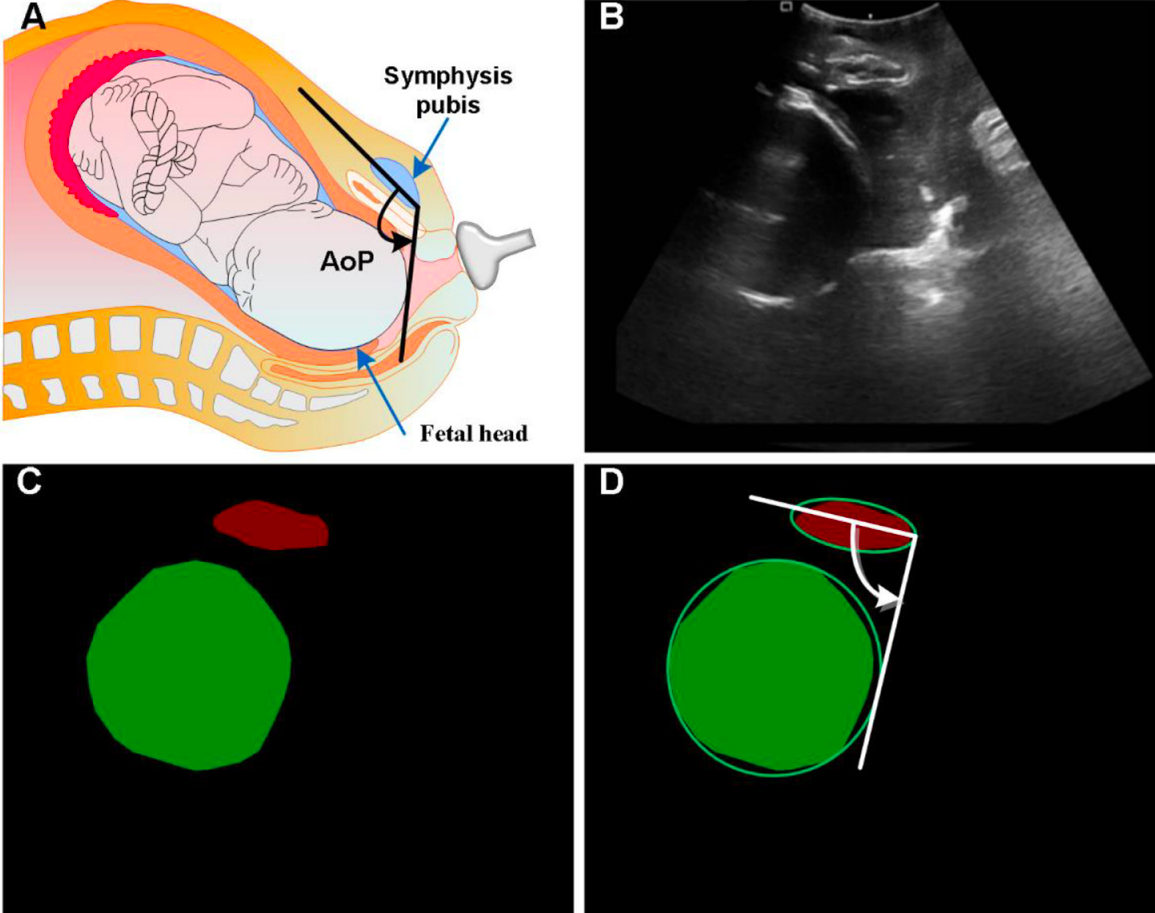
\includegraphics[width=\linewidth]{explanation}
        \vspace{-7mm}
        \caption{Assessment of FD in the birth canal by measurement AoP}
    \end{figure}
    \small
    \vspace{-5mm}
    \textbf{Data ~\cite{LU2022107904}:}
    4000 MHA files for image data ($3\times256\times256$)
    and for labels ($256\times256$, pixels labeled as 
    0 - bg, 1 - PS, or 2 - FH).

    \textbf{Goal:}
    Segmentation algorithms, predicting images ($256\times256$) containing
    labeled pixels.


    \column{0.5\textwidth}
    \small
    \begin{itemize}
        \item \textit{Risk:} maternal and perinatal morbidity 
        \item \textit{Pathology:} longer labor duration 
        (slow progression of fetal descent(FD))
        \item \textit{Accurate assessment} of FD by 
        monitoring the FH station \textit{remains challenge} 
        in guiding obstetric management
        \item Manual segmentation of SP-FH from transperineal US (TPU)
        images is the most reliable, but \textit{extremely time-consuming} 
        \item Automatic measurement algorithms based on AI are 
        expected to be \textit{efficient, reproducible and objective} 
    \end{itemize}
    \end{columns}
\end{frame}


\section{Challenge Results}

%---------------------------------------------------------

\begin{frame}
    \frametitle{Metrics and Results}
\normalsize
\resizebox{\textwidth}{!}{
\begin{tabular}{cccccccccccc}
\hline
\textbf{Team}           & \textbf{AoP}       & $\mathbf{HD_{FH}}$   & $\mathbf{HD_{PS}}$   & $\mathbf{MSD_{FH}}$  & $\mathbf{MSD_{PS}}$  & $\mathbf{HD_{ALL}}$  & $\mathbf{MSD_{ALL}}$ & $\mathbf{DICE_{FH}}$ & $\mathbf{DICE_{PS}}$ & $\mathbf{DICE_{ALL}}$ & \textbf{Score}  \\
\hline
Gregor Koe     & 6.544     & 12.631    & 7.638   & 3.896   & 2.409   & 13.448   & 3.486   & 0.930   & ??      & 0.924    & 0.9418 \\
\rowcolor[RGB]{247,203,184}
Marawan Elbatel  & 7.970     & 10.699    & 7.559   & 3.307  & 2.995   &12.059   &2.981     & 0.940 & ??      &0.935 & 0.9416 \\
Yaoyang Qiu    & 7.647     & 12.459    & 7.661   & 3.616   &2.257  & 13.615   & 3.238   & 0.936   & ??      & 0.930    & 0.939  \\
Gongping Chen  & 8.558     & 14.011    & 9.051   & 3.869   & 2.620   & 15.334   & 3.517   & 0.931   & 0.860   & 0.924    & 0.931  \\
\rowcolor[RGB]{247,203,184}
Fangyijie Wang & 8.719     & 14.009    & 10.829  & 3.984   & 2.982   & 15.809   & 3.579   & 0.931   & 0.858   & 0.925    & 0.928  \\
\rowcolor[RGB]{247,203,184}
Hongkun Sun  & 9.276     & 15.795    & 11.536  & 4.723   & 3.114   & 17.560   & 4.265   & 0.918   & 0.831   & 0.910    & 0.923  \\
\rowcolor[RGB]{247,203,184}
Pengzhou Cai  & 12.199    & 20.031    & 14.068  & 7.099   & 4.208   & 21.873   & 6.058   & 0.879   & 0.804   & 0.872    & 0.897  \\
YuboTan        & 14.048    & 16.041    & 16.023  & 5.199   & 7.260   & 20.251   & 5.106   & 0.910   & ??      & 0.894    & 0.892  \\
\hline
\end{tabular}
}
\footnotesize
\textit{*The participants for whom model information is 
available are highlighted in color}
\small
\begin{itemize}
\setlength{\itemsep}{0.2em} % Adjust the vertical spacing between items
\setlength{\leftmargin}{0em} % Adjust the left indent
    \item \textbf{Dice Coefficient}
    $D C=\dfrac{2 \times\left|I_P \cap I_L\right|}{\left|I_P\right|+\left|I_L\right|},$
where $I_P$ is the model prediction, 
$I_L$ is the ground truth, and $|\cdot|$ is the number of pixels 
belonging to the object.

    \item  \textbf{Hausdorf  Distance}
    $H D=\max \left\{\sup _{x \in  I_P} \inf _{y \in I_L} d(x, y), \sup _{y \in I_L} \inf _{x \in I_P} d(x, y)\right\}$,
    where $d(x, y)$ is the distance between points $x$ 
    and $y$. 
    \item  \textbf{Mean Surface Distance} 
    $\mathrm{MSD}=\dfrac{1}{\left|I_P\right|+\left|I_L\right|}\left(\sum_{x \in I_P} d\left(x, I_L\right)+\sum_{y \in L} d\left(y, I_P\right)\right)$

    \item $\mathbf{\Delta A o P}=\left|A o P_P-A o P_L\right|,$
    where $A o P_P$ represents the predicted magnitude, 
    and $A o P_L$ is the magnitude of the labeled AoP. 
    
    \item $\mathbf{Score} = 0.5\left(1-\dfrac{\Delta AoP}{180}\right)+
    0.25\dfrac{DICE_{FH}+DICE_{PS}+DICE_{ALL}}{3}+
    0.25\left[0.5 \left(1- \dfrac{HD_{FH}+HD_{PS}+HD_{ALL}}{3 \times 100} \right)+
    0.5 \left(1- \dfrac{MSD_{FH}+MSD_{PS}+MSD_{ALL}}{3 \times 100} \right)\right]$
\end{itemize}
\end{frame}

\begin{frame}
    \frametitle{Methods and Results}
    \resizebox{\textwidth}{!}{
        \begin{tabular}{cccccccccccc}
        \hline
        \textbf{Team}           & \textbf{AoP}       & $\mathbf{HD_{FH}}$   & $\mathbf{HD_{PS}}$   & $\mathbf{MSD_{FH}}$  & $\mathbf{MSD_{PS}}$  & $\mathbf{HD_{ALL}}$  & $\mathbf{MSD_{ALL}}$ & $\mathbf{DICE_{FH}}$ & $\mathbf{DICE_{PS}}$ & $\mathbf{DICE_{ALL}}$ & \textbf{Score}  \\
        \hline
        Gregor Koe     & 6.544     & 12.631    & 7.638   & 3.896   & 2.409   & 13.448   & 3.486   & 0.930   & ??      & 0.924    & 0.9418 \\
        \rowcolor[RGB]{247,203,184}
        Marawan Elbatel    & 7.970     & 10.699    & 7.559   & 3.307  & 2.995   &12.059   &2.981     & 0.940 & ??      &0.935 & 0.9416 \\
        Yaoyang Qiu    & 7.647     & 12.459    & 7.661   & 3.616   &2.257  & 13.615   & 3.238   & 0.936   & ??      & 0.930    & 0.939  \\
        Gongping Chen  & 8.558     & 14.011    & 9.051   & 3.869   & 2.620   & 15.334   & 3.517   & 0.931   & 0.860   & 0.924    & 0.931  \\
        \rowcolor[RGB]{247,203,184}
        Fangyijie Wang  & 8.719     & 14.009    & 10.829  & 3.984   & 2.982   & 15.809   & 3.579   & 0.931   & 0.858   & 0.925    & 0.928  \\
        \rowcolor[RGB]{247,203,184}
        Hongkun Sun  & 9.276     & 15.795    & 11.536  & 4.723   & 3.114   & 17.560   & 4.265   & 0.918   & 0.831   & 0.910    & 0.923  \\
        \rowcolor[RGB]{247,203,184}
        Pengzhou Cai  & 12.199    & 20.031    & 14.068  & 7.099   & 4.208   & 21.873   & 6.058   & 0.879   & 0.804   & 0.872    & 0.897  \\
        YuboTan        & 14.048    & 16.041    & 16.023  & 5.199   & 7.260   & 20.251   & 5.106   & 0.910   & ??      & 0.894    & 0.892  \\
        \hline
        \end{tabular}
        }
        \footnotesize
        \textit{*The participants for whom model information is 
        available are highlighted in color}
         
        \small
        \begin{itemize}
            \item \textbf{Marawan Elbatel ~\cite{MarawanElbatel}:} 
            pre-trained \href{https://segment-anything.com/}{Segment Anything Model (SAM)} 
            by \textbf{Meta AI} (freezing the model and performing 
            low-ranked fine-tuning of the image encoder)

            \item \textbf{Fangyijie Wang ~\cite{FangyijieWang}:}
            U-Net-based segmentation model from the 
            \href{https://pypi.org/project/segmentation-models-pytorch/}{Segmentation Models SPM} 
            library

            \item \textbf{Hongkun Sun ~\cite{hongkunsun}:}
            Custom NN model which is a combination of several 
            architectural components, including ResNet, 
            Multi-Scale Attention Blocks, ViT (Vision Transformer) blocks, 
            and various convolutional and transposed convolutional layers

            \item \textbf{Pengzhou Cai ~\cite{cai2023pubic}:}
            Custom method, named BRAU-Net, adopting a U-Net-like
            pure Transformer architecture with bi-level routing 
            attention and skip connections
            \end{itemize}
\end{frame}


\section{FH-PSSNet Model}
%---------------------------------------------------------
\begin{frame}
    \frametitle{Architecture}
    The FH-PSSNet model ~\cite{organizers} is based on an encoder-decoder
    framework, incorporating a dual attention module, a multi-scale feature screening module and a
    direction guidance block. 
    \vspace{-3mm}
    \begin{figure}[H]
        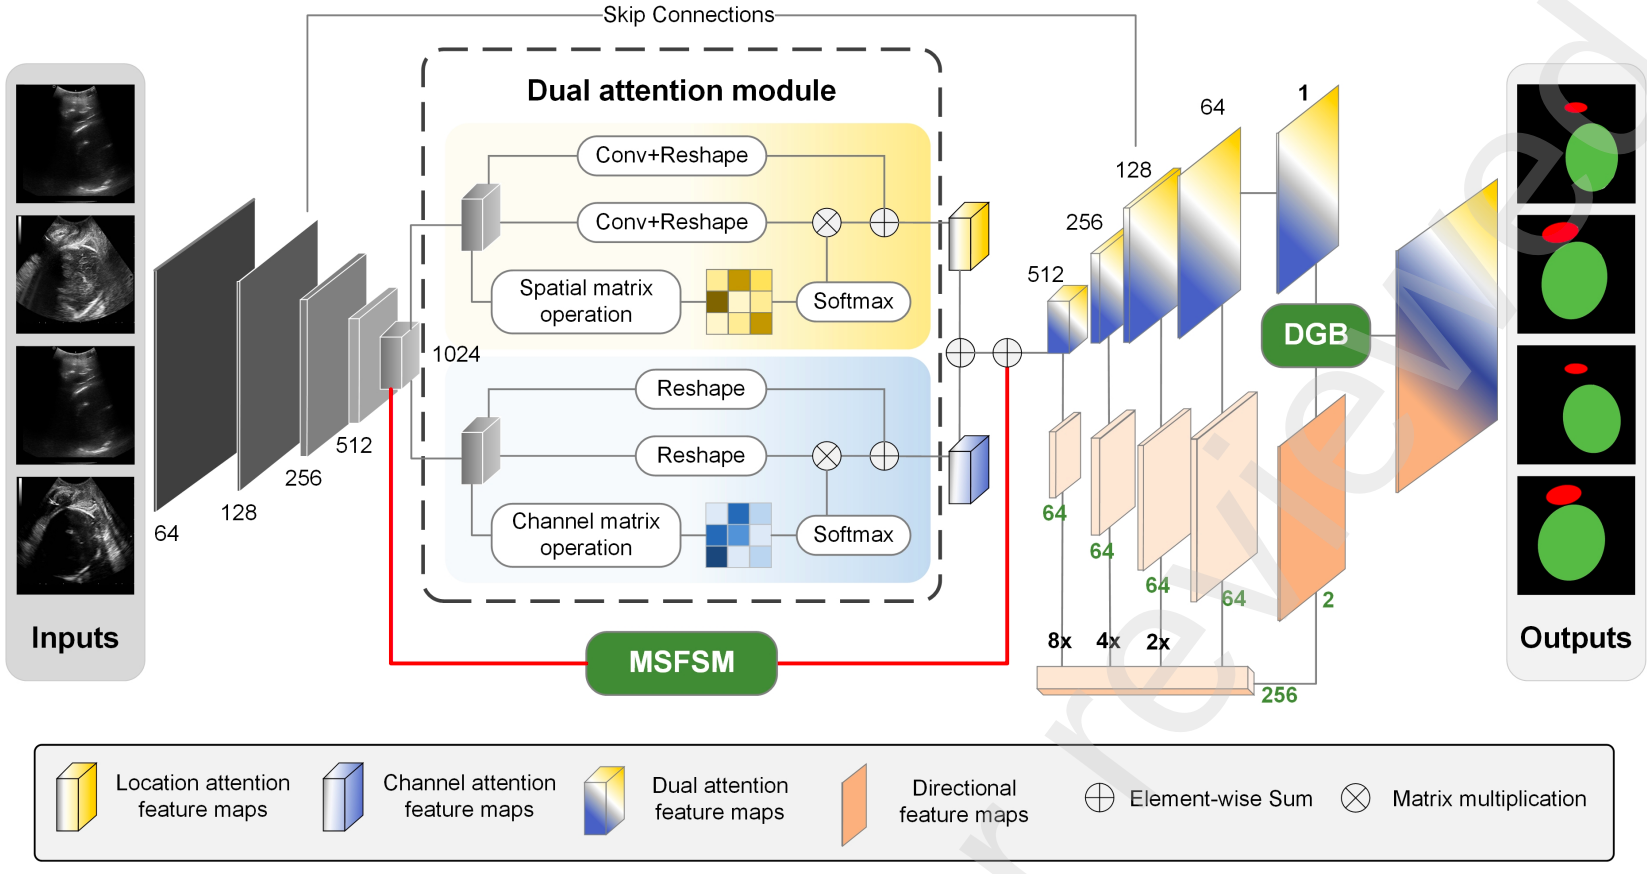
\includegraphics[width=0.9\linewidth]{fhpssnet}
        \vspace{-2mm}
        \caption{The overall framework of the model}
    \end{figure}

\end{frame}

%---------------------------------------------------------
%Two columns
\begin{frame}
\frametitle{Performance and Comparison with Other Models}

\begin{columns}
\column{0.4\textwidth}
\vspace{-6mm}
\begin{figure}[H]
    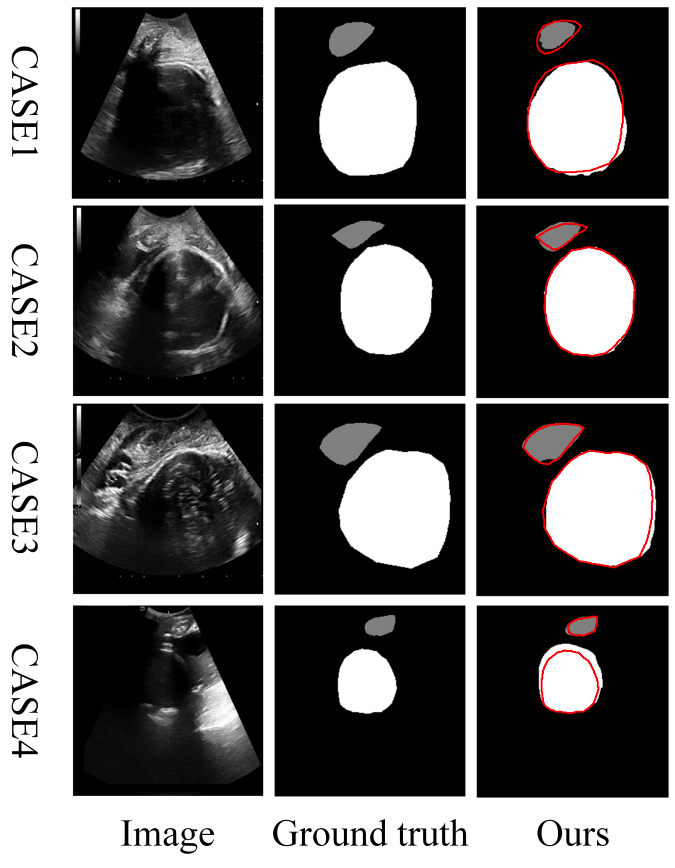
\includegraphics[width=0.96\linewidth]{performance}
    \vspace{-2mm}
    \caption{The performance of the FH-PSSNet model}
\end{figure}

\column{0.6\textwidth}
\centering
\small
\begin{tabular}{c|cc|cc}
    \hline Model name & \multicolumn{2}{c|}{ FH } & \multicolumn{2}{c}{ PS } \\
    \hline & DC $\uparrow$ & HD $\downarrow$ & DC $\uparrow$ & HD $\downarrow$ \\
    \hline SegNet & 0.917 & 3.740 & 0.821 & 4.011 \\
    DeepLab & 0.917 & 3.745 & 0.823 & 4.020 \\
    FCN & 0.921 & 3.481 & 0.850 & 3.699 \\
    U-Net & 0.932 & 3.538 & 0.855 & 3.852 \\
    AU-Net & $\mathbf{0.938}$ & 3.404 & 0.867 & 3.570 \\
    DAG V-Net & 0.933 & 3.393 & 0.866 & $\mathbf{3.560}$ \\
    FDA & 0.929 & 3.408 & 0.863 & 3.574 \\
    \mybox{FH-PSSNet} & $\mathbf{0.938}$ & $\mathbf{3.390}$ & $\mathbf{0.870}$ & $3.562$ \\
    \hline
\end{tabular}

\vspace{6mm}

The best performance of challenge participants:

\vspace{3mm}

\begin{tabular}{cc|cc}
    \hline  \multicolumn{2}{c|}{ FH } & \multicolumn{2}{c}{ PS } \\
    \hline  DC $\uparrow$ & HD $\downarrow$ & DC $\uparrow$ & HD $\downarrow$ \\
    \hline  0.940 & 10.699 & 0.860 & 7.559 \\
    \hline
\end{tabular}
\end{columns}

\end{frame}



%---------------------------------------------------------

\section{References}

\begin{frame}
  \frametitle{References}
  \printbibliography % This command will generate the list of references
\end{frame}



\begin{frame}
    \Large
    \begin{alertblock}{}
        \centering
        Thank you for your attention!

        Any questions?
    \end{alertblock}
\end{frame}

\end{document}
